
%Diese LaTeX-Vorlage f�r Praktikumsprotokolle in Form einer Ver�ffentlichung f�r das 
%F-Praktikum wurde erstellt von Andreas Nuber EP II, Uni W�rzburg.
%Es wurde das Koma-Skript verwendet und sollte somit installiert sein
%desweiteren sollten alle packages installiert sein, die mit \usepackage{} 
%eingebunden werden.
%Zum Testen dieser Vorlage wurde MikTex verwendet sowie TeXnicCenter als Editor
%beim Compilieren waren 0 Fehler, 1 Warnung und 3 zu volle/leere Boxen. Das ist ok :)

%F�r das Erstellen einfach den sinnfreien Text, der zum ausf�llen genommen wurde 
%ersetzen. Was sonst noch ver�ndert werden sollte steht in den Kommentaren!


\documentclass[a4paper,10pt,twocolumn]{scrartcl} %Koma-Skript-�quivalent zu "article"

\usepackage{german}            %macht deutsche �berschriften
\usepackage[latin1]{inputenc}  %man kann Sonderzeiche wie �,� usw direkt eingeben
\usepackage{amsmath}           %macht
\usepackage{amsfonts}          %Mathe
\usepackage{amssymb}           %m�chtiger
\usepackage{graphicx}          %erlaubt Graphiken einzubinden (.eps f�r dvi und ps sowie .jpg f�r pdf)
\usepackage[T1]{fontenc}       %Zeichenbelegung der verwendeten Schrift
\usepackage{ae}                %macht sch�neres �
\usepackage{typearea}	       %erm�glicht �nderung des Seitenspiegels
\usepackage{scrlayer-scrpage}  %erm�glicht �nderung der Kopf-/Fu�zeile
\usepackage{lastpage}          %l�sst auf die Seienanzahl zugreifen
\usepackage[margin=10pt,font=small,labelfont=bf]{caption} %macht die Bildbeschriftungen richtig
\usepackage{siunitx}
\usepackage{url}
\usepackage{placeins}
\usepackage[nodayofweek]{datetime} 
\usepackage{textgreek}
\usepackage{caption}
\usepackage{cuted}

%\renewcommand{\figurename}{Abb.}

\pagestyle{scrheadings}        %sagt Koma-Skript, dass selbstdefiniers Kopfzeilen verwendet werden
\typearea{16}                  %stellt Seitenspiegel ein
\columnsep25pt				   %definiert Breite zwischen den zwei Spalten von \twocolumns

\renewcommand{\pnumfont}{%     %�ndert die Schriftart der Seitennummerierung
\normalfont\rmfamily\slshape}  %�ndert die Schriftart der Seitennummerierung 
\renewcommand\refname{References}
\renewcommand{\figurename}{Fig.}
\renewcommand{\tablename}{Tab.}

\begin{document}
\cfoot{\thepage /\pageref{LastPage}}     %macht die Seitennumerierung der Fom 2/5 (ausser auf der Titelseite)

\twocolumn[{\csname @twocolumnfalse\endcsname                %erlaubt "Abstrakt" �ber beide Spalten
\titlehead{                                                  %Kopfzeile
	\begin{tabular*}{\textwidth}[]{@{\extracolsep{\fill}}lr}   %Kopfzeile
	Instructor: Tobias Kie�ling & \today\\                          %Kopfzeile      hier den Betreuer eintragen!!!
	\end{tabular*}                                             %Kopfzeile
	}
\title{Measuring Planck's constant via photoeffect and Boltzmann's constant through a transistor collectorcurrent}	    %Titel der Versuchs
\author{Jonas Beck and Jonathan Bodky		}                   %Namen der Studenten
\date{}                                                         %ben�tigt um automatisches Datum auszuschalten
\maketitle                                                      %erzeugt Titelseite
\vspace{-8ex}                                                   %verringert Abstand zur �berschrift
\begin{abstract}                                                %Beginn des Abstracts
We use the photoelectric effect to measure Planck's constant as $h=(5,75\pm 0,51)\cdot 10^{-34}\,\si Js$ by evaluating the slope of the maximal photoelectron energies over the frequency of the used light via Einstein's equation. We also measure Boltzmann's constant at different temperatures via the diffusion current through a pn-transition in a transistor. This current is proportional to a Boltzmann factor, such that by fitting our data with an exponential we can read off Boltzmann's constant as $k_\text B=(1,3777 \pm 0,0012)\cdot 10^{-23}\,\frac{\si\J}{\si\K}$.
\\ \\ 
\\ 
Executed: 1\textsuperscript{st} December, 2021\\       %Datum �ndern!
First submission: 8\textsuperscript{th} December, 2021\\ 	%Datum �ndern!
Second submission: 19\textsuperscript{th} January, 2022
\\ 
\\ 
\end{abstract}
}]

\section{Introduction}
Planck's and Boltzmann's constants are two of the most important fundamental constants in physics. The Boltzmann constant $k_\text B$ describes the connection between energy and temperature and is used to model all kinds of thermodynamic systems. Here, due to the big number of degrees of freedom, it usually is not possible to describe all of them one by one. Often a statistical approach via temperature and Boltzmann's constant is neccesary.
Planck's constant $h$ on the other hand appears almost everywhere in quantum mechanics. It has great philosophical significance as the minimum resolution of phase space in Heisenberg's uncertainty principle, while its numerical value is just as important as it links an objects frequency to its energy.\\
Both constants are used in modern metrology to define the SI-unit system, so they have been given exact defining values. But of course, we can still try to measure them with the methods available and compare results, which is the goal of this paper.

\section{Measuring Planck's constant}
\subsection{The photoelectric effect}
To determine the value of Planck's constant, we use the photoeffect, which will be described briefly in this section.\\\\
The photoeffect occurs when photons with  sufficient energy $E_\text{ph}=h\nu$ hit the electrons in an atom. In that case, they can be absorbed, giving their energy to the electron. The electron now has enough kinetic energy to leave the bound state of the atom and after overcoming the work function $W_\text A$ of the material the atom was part of, the electron now travels through space as a free particle with the remaining energy
\begin{align}\label{eq:einstein}
E_\text{e}=h\cdot \nu-W_\text A
\end{align}
as was discovered by Einstein in 1905 \cite{gerth}. This energy can be measured by applying an opposing electric field and measuring the current, thus the number of electrons overcoming this field. This is exactly how a photo cell such as the one used in our experiment works. Photons release electrons from the cathode and those with high enough energy overcome the counter voltage between cathode and anode and can be detected as a photocurrent.

\subsection{Experimental setup and analysis of the Planck data}
\begin{figure}[htbp]
\begin{center}
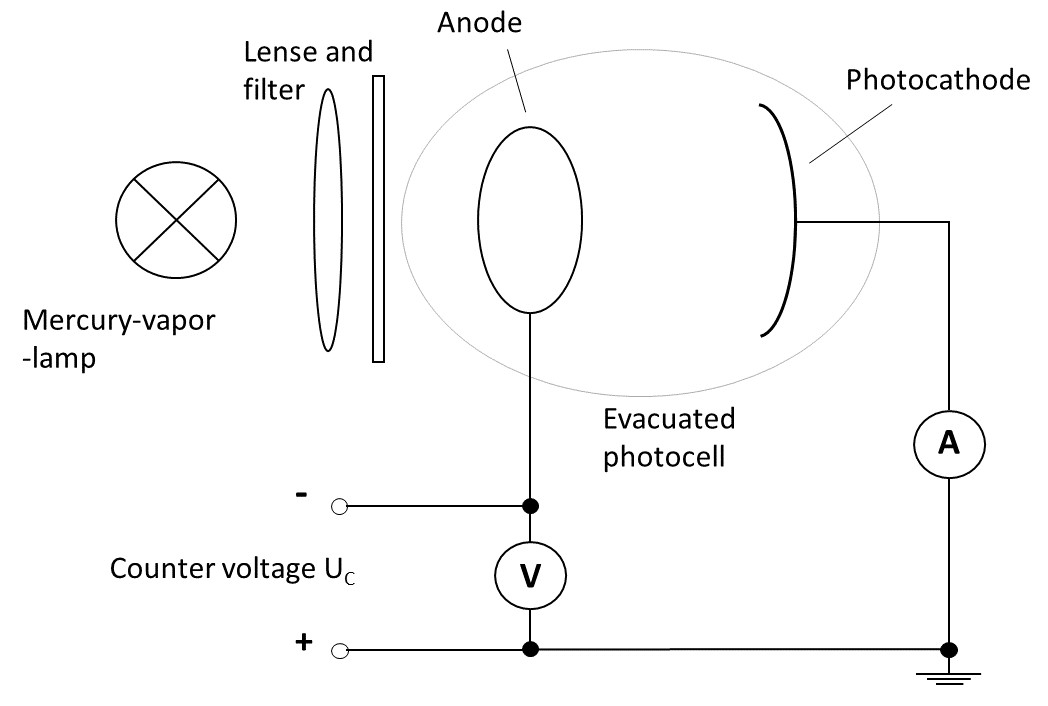
\includegraphics[width=\columnwidth]{img/Planck-Schaltkreis}
\end{center}
\caption[]{Experimental setup to measure Planck's constant: Light from a Hg-lamp is focused with a lens onto the cathode of a photo cell, passing an interference filter on the way. The current at the cathode is then measured for different countervoltages between cathode and anode.}
\label{fig:planck-setup}
\end{figure}
The experimental setup that was available is shown in Fig.~\ref{fig:planck-setup} and consists of a photo cell, a Hg-lamp to supply the photons, interference filters of various wavelengths to select only discrete wavelengths of light and a lens to focus the beam on the cathode as well as an \grqq Agilent 34405A \grqq -voltmeter and a \grqq Keithley 6485 Picoammeter \grqq -amperemeter.\\
We measured the photocurrent in dependence of the counter voltage for five wavelenghts in the visible spectrum. In each of these five curves we interpolate the voltage where the photocurrent is detectable against the underground, which is mostly caused by an opposing photoeffect due to pollution on the platinum anode: As platinum has a sufficiently large work function, in an ideal setup there would be no opposing photoeffect and the anode current would tend to zero for large enough counter voltages. In reality there are impurities at the cathode with a smaller work function, leading to an opposing photocurrent, which shifts the measured characteristic curve down (with a larger shift for larger countercurrents) and can be approximated by a linear function~\cite{instr}. A more detailed description of the interpolation method can be found in the appendix at section~\ref{sec:planck-int}, the plots can be found in Fig.~\ref{fig:planck-prim1} and~\ref{fig:planck-prim2-5}. At those interpolated counter voltages, only the electrons moving straight towards the anode can overcome the electric field, and thus the energy of the photoelectrons can be calculated.
\begin{figure}[htbp]
\begin{center}
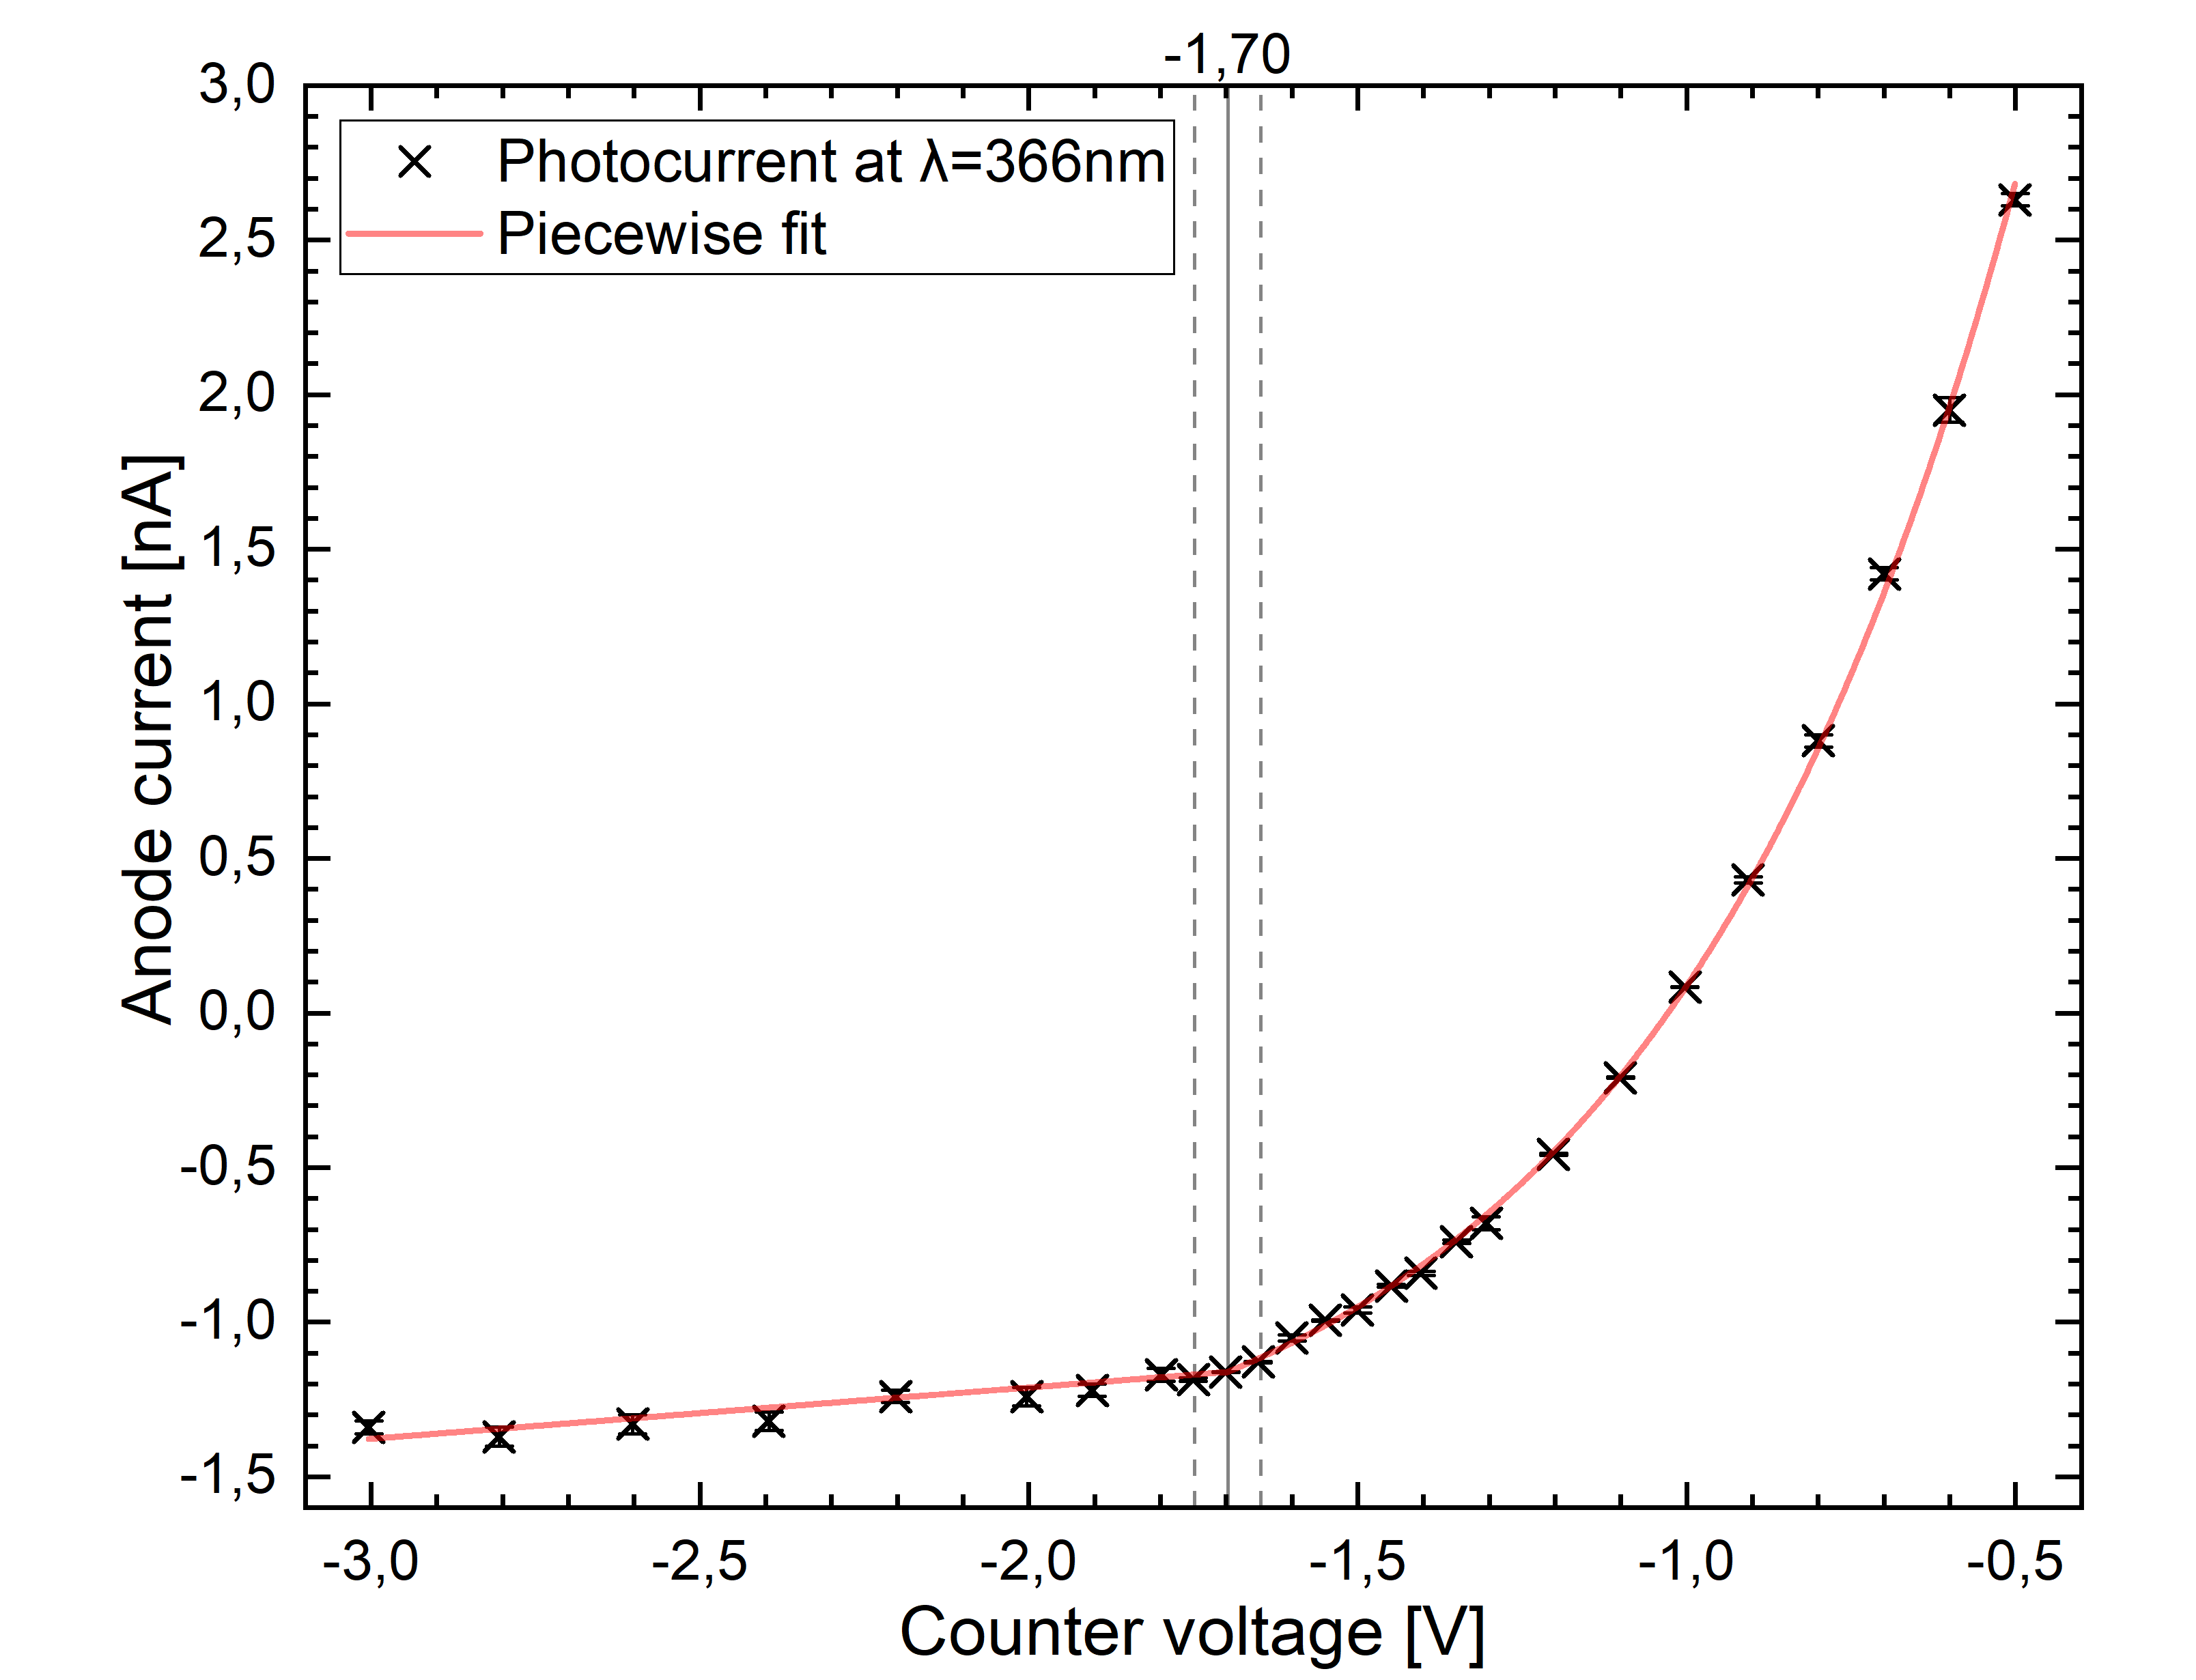
\includegraphics[width=\columnwidth]{img/Kennlinie-366}
\end{center}
\caption[]{Photocurrent in dependence of the countervoltage for light of wavelength $\lambda= 366 \,\si\nm$. A piecewise, first linear and then exponential, function was fitted to the data to determine the point where the relevant signal is detectable against the underground. This is at the transition point between the two functions.}
\label{fig:planck-prim1}
\end{figure} 
\begin{table}[htbp]          %so funktionieren die Tabellen in LaTeX
\centering
\begin{tabular*}{\linewidth}{@{\extracolsep{\fill}}cc}
\hline
\hline
\rule[-7pt]{0pt}{23pt}  frequency $\nu$ [$10^{14}\,\si{\Hz}$]  &  counter voltage $U_G$ [$\si{\V}$]  	 \\
\hline
\rule[-5pt]{0pt}{23pt}   $5,19 \pm 0,05$   &   $-0,6 \pm 0,1$  	 \\
\rule[-5pt]{0pt}{23pt}   $5,49 \pm 0,05$   &   $-0,7 \pm 0,1$  	 \\
\rule[-5pt]{0pt}{23pt}   $6,88 \pm 0,07$   &   $-1,24 \pm 0,08$  	 \\
\rule[-5pt]{0pt}{23pt}   $7,40 \pm 0,07$   &   $-1,38 \pm 0,06$  	 \\
\rule[-5pt]{0pt}{23pt}   $8,19 \pm 0,08$   &   $-1,70 \pm 0,05$  	 \\
\hline
\hline
\end{tabular*}  
\normalsize
\caption[]{Countervoltages where the fastest photoelectrons can just overcome the electric field, in dependence of the frequency of the light used to cause the photoeffect.}  %siehe Graphik: Beschriftung
\label{tab:countervoltages}                             %siehe Graphik: zum Zitieren
\end{table}
\\
Now we can plot these voltages shown in Tab.~\ref{tab:countervoltages} against the frequencies of the light at which they were measured and use Einstein's equation (eq.~\ref{eq:einstein}) to receive Planck's constant with the slope $m$ of a regression line through that plot (Fig.~\ref{fig:planck-secundary}) as
\begin{align}
h=m\cdot e
\end{align}
with the elementary charge $e=1,602176634\cdot 10^{-19}\,\si{C}$ \cite{codata}. We estimated the relative error of the frequencies to be $1\%$ as there is no information available about the interference filters.\\\\
\begin{figure}[htbp]
\begin{center}
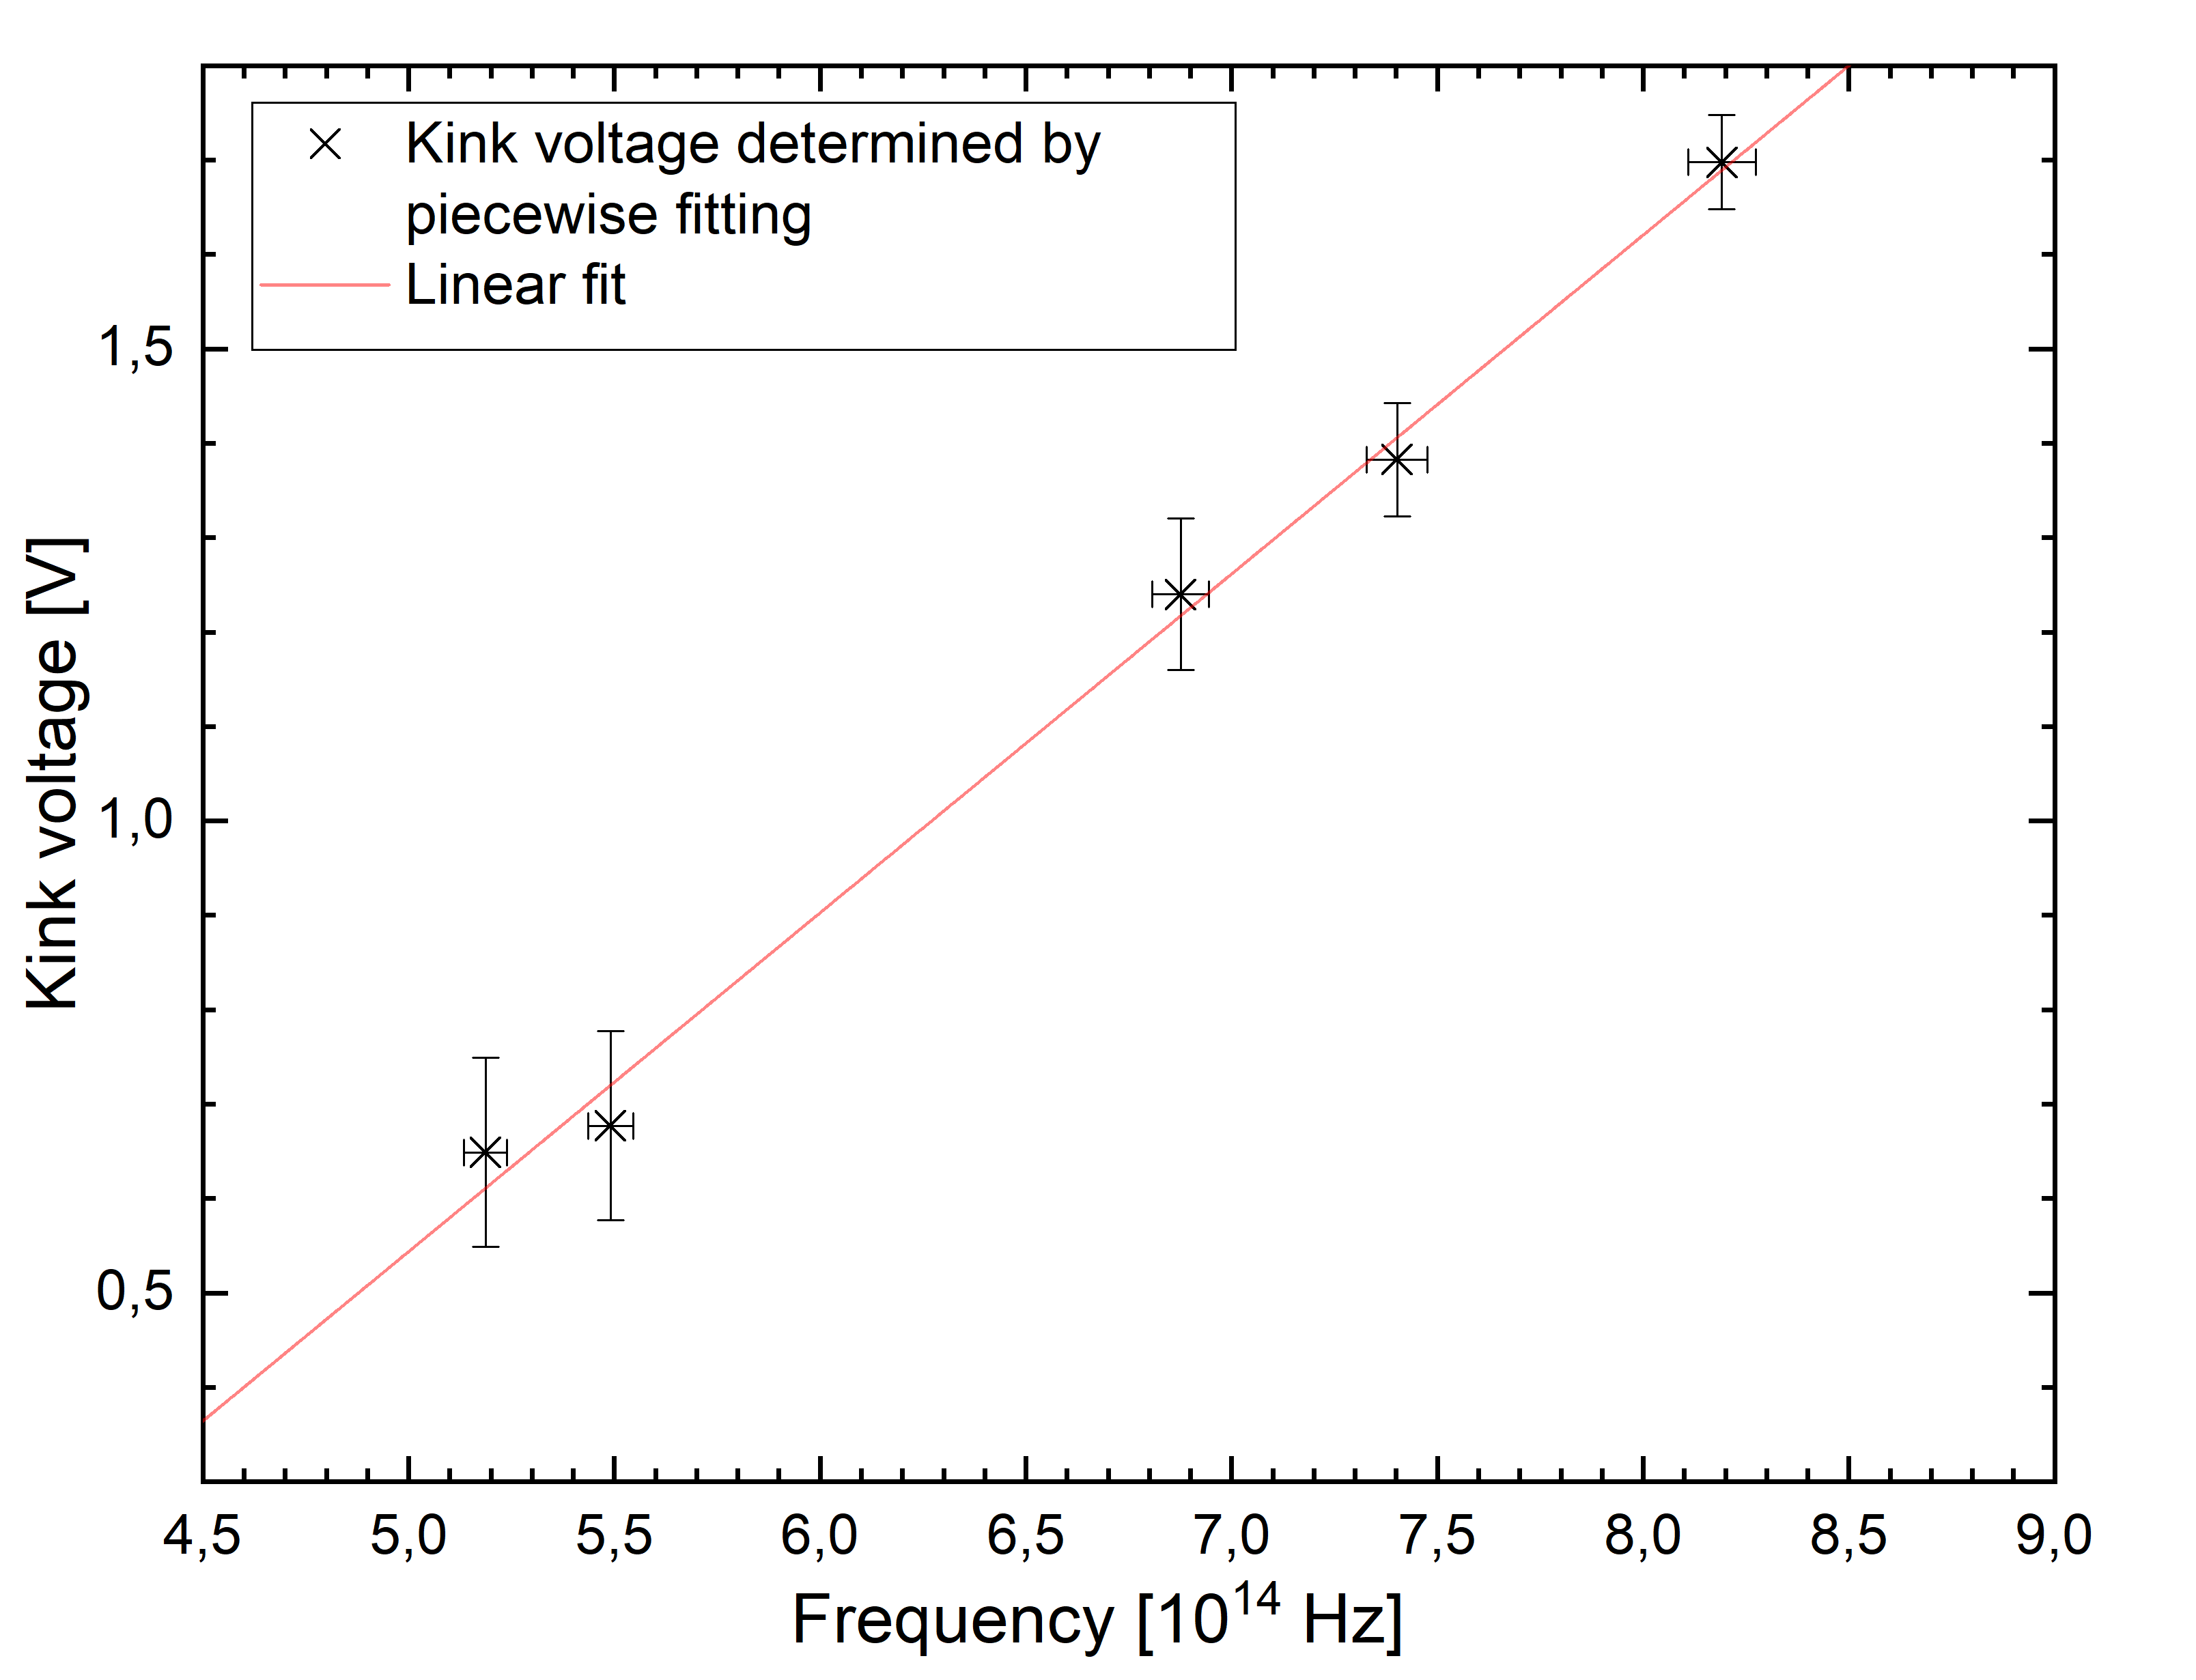
\includegraphics[width=\columnwidth]{img/PlanckKonstante}
\end{center}
\caption[]{Maximal countervoltages in dependence of the frequency of the light causing photoeffect. According to Einstein's equation, this data in theory follows a line with slope $\frac{h}{e}$.}
\label{fig:planck-secundary}
\end{figure} 
\\With this method, we receive $h~=~(5,75~\pm~0,51)~\cdot ~10^{-34}\,\si Js$. This value coincides with the exactly defined value of $h_\text{exact}=6.626 070 15\cdot 10^{-34}\,\si Js$ \cite{codata} within a two-sigma errorinterval. Our error can not really be thought of as a statistical gaussian error, as we did not have enough datapoints for that. That our value deviates from the theoretical value by $13\%$ can also be explained with the small dataset and pollution on the anode: with more datapoints, the maximum counter voltage the electrons can overcome could have been localised better, and with less pollution there should be less underground signal, leading again to a better localisation of the maximum counter voltages.


\section{Measuring Boltzmann's constant}
\subsection{Shockley equation for the current through a pn-transition}
In order to measure Boltzmann's constant we use a semiconductor pn-transition as can be found in transistors and diodes. At such a transition there always is an exchange of electrons due to thermodynamic effects and thus there are (opposing) currents, even if no voltage is applied. As those currents of course are in thermal equilibrium, they are related to Boltzmann's constant und thus we can use them to determine the latter.\\\\
The net current at such a transition can be described with the Schockley equation, which will be motivated in this paragraph. At the transition from n- to p-doped semiconductor positive and negative charge carriers will meet and recombine due to diffusion, so there is a zone without free charge carriers where only the oppositely charged ions remain. They create a potential difference opposing the direction of diffusion, the so called antidiffusion voltage $U_A$.
As the system is at finite temperature, some bound electrons in the carrier free zone are statistically excited from the valence into the conduction band and can then be accelerated by the antidiffusion voltage, creating an intrinsic current $I_0$ opposite to the direction of diffusion. On the other hand, some diffusing charge carriers are fast enough to overcome the antidiffusion voltage, resulting in the diffusion current $I_D$. To do so, they must have a kinetic energy of $E\geq e\cdot U_\text A$ where $e$ is the elementary charge. And as the energy of the electrons in the conduction band follows Boltzmann statistics, the diffusioncurrent is proportional to a Boltzmann factor
\begin{align}\label{eq:schockley1}
 I_\text{D,0}\sim e^{-\frac{e\,U_\text A}{k_\text B\,T}}.
\end{align}
As in thermal equilibrium without an outer voltage there should be no current, it follows that 
\begin{align}
|I_\text{D,0}|=|I_\text 0|.
\end{align}
If we now apply an outside voltage at the transition, the anti diffusion voltage is decreased by that voltage and because of eq.~\ref{eq:schockley1} we get
\begin{align}\label{eq:schockley0}
I_\text D(U)=I_\text{D,0}\cdot e^{\frac{e\,U}{k_\text B\,T}}=I_\text 0\cdot e^{\frac{e\,U}{k_\text B\,T}}
\end{align}
and for the total current by subtracting the intrinsic current itself, which is not changed by the applied voltage:
\begin{align}
I_\text{tot}(U)=I_\text 0\cdot \big(e^{\frac{e\,U}{k_\text B\,T}}-1\big)
\end{align}
The last equation is known as Schockley's equation \cite{instr}. But as this is only a simple model, in reality there will be other currents flowing along the crystal boundaries and interfering with the measurement. We can however compensate these disturbances by symmetrically adding a second pn-transition - which just transforms the diode into a transistor. There, the additional currents as well as the intrinsic current of the transitions cancel out, as they are added at one transition and subtracted again at the other, while our diffusion current from the first transition will pass the second one almost completely as it flows in transmission direction of the second diode. So we do not even need the real Schockley equation, but just eq.~\ref{eq:schockley0} to describe the collector current in dependence of an applied basis-emitter voltage \cite{instr}.

\subsection{Experimental setup and analysis of the Boltzmann data}
\begin{figure}[htbp]
\begin{center}
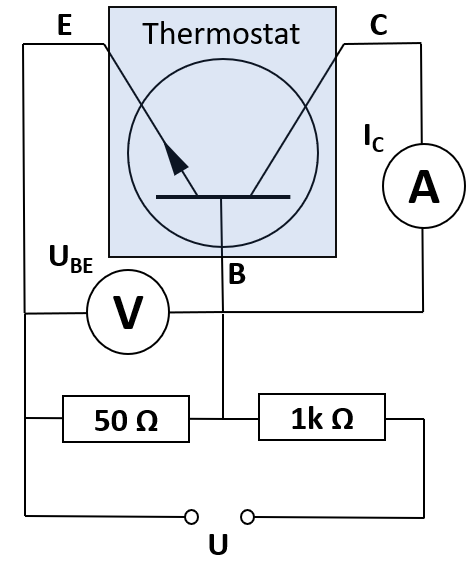
\includegraphics[width=\columnwidth]{img/Boltzmann-Schaltkreis}
\end{center}
\caption[]{Experimental setup to measure Boltzmann's constant: Via a voltage divider circuit, a voltage is applied to the base-emitter transition of a npn-transistor which is kept at a specific temperature by a thermostat. The collectorcurrent is measured in dependence of this current, following a Boltzmann factor so we can calculate Boltzmann's constant.}
\label{fig:boltzmann}
\end{figure}
A circuit diagram of our setup is shown in Fig.~\ref{fig:boltzmann}. As transistor, we used a \grqq npn-Leistungstransistor 2N 3055\grqq. The outside voltage was applied to the emitter-base np-transition from a \grqq zentro electric\grqq ~power supply via a voltage divider circuit and was measured with an \grqq Agilent 34405A\grqq multimeter. The same applies for the collectorcurrent, which as argued above is in good approximation the diffusion current from eq.~\ref{eq:schockley0}. During these measurements, the transistor was kept at a specific temperature with a \grqq Lauda Ecoline Startedition RE104\grqq ~thermostat.
\begin{figure}[htbp]
\begin{center}
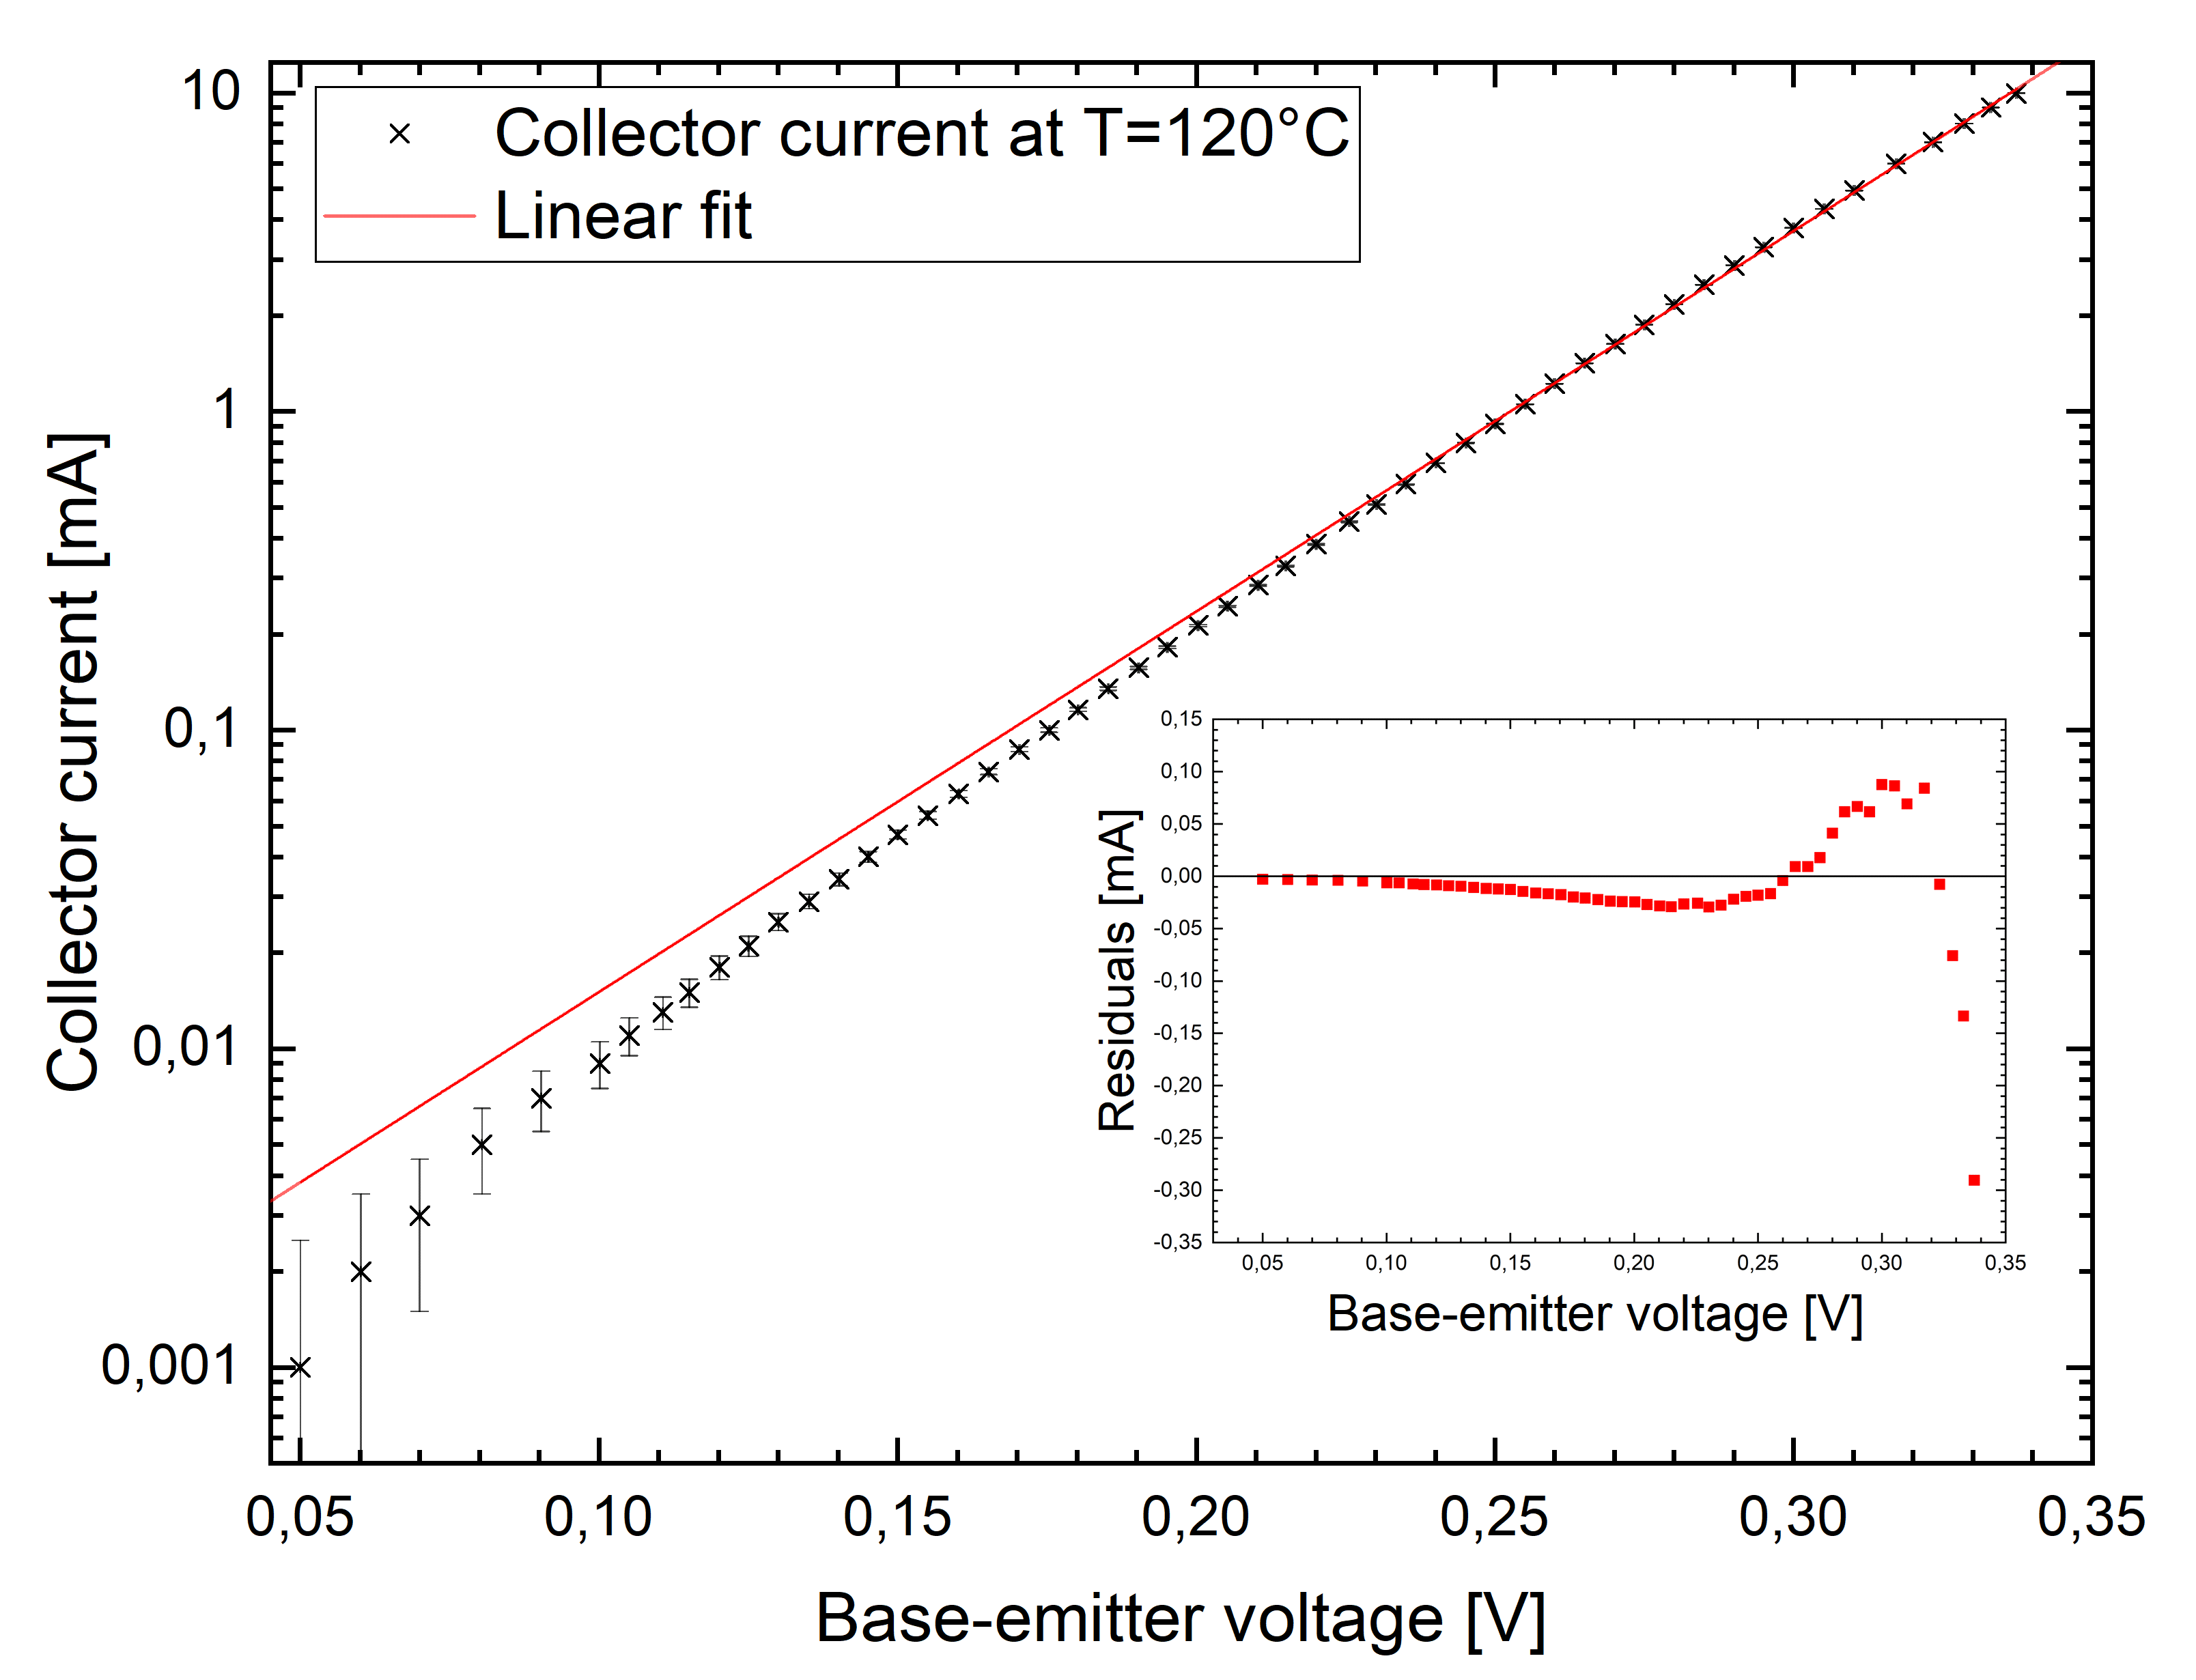
\includegraphics[width=\columnwidth]{img/120C_Kennlinie_unk}
\end{center}
\caption[]{Collector current in dependence of the base-emitter voltage at temperature $T=120\,\si\celsius$ in logarithmic application with a linear fit function and residuals in the inset. For small and large values the data clearly deviates from the theoretical expection, giving rise to the assumption that there must be a yet untreated systematic error in the measurement.}
\label{fig:boltzmann-120u}
\end{figure}
We measured the $I(U)$-curves for the three temperatures $T_1=40\,\si\celsius$, $T_2=80\,\si\celsius$ and $T_3=120\,\si\celsius$. The data was then fitted with an exponential function, an example of which in logarithmic application is displayed in Fig.~\ref{fig:boltzmann-120u}. As can be seen from the residuals, for small and big voltages there is a quite significant systematic error, as the data does not follow the expected exponential very well. This is due to the non negligible resistance $R$ of the emitter, which decreases the effectively applied basis-emitter voltage. This resistance can be compensated by modifying eq.~\ref{eq:schockley0} to
\begin{align}
I_\text C(U)=I_\text 0\cdot e^{\frac{e\,(U-R\,I_\text C(U))}{k_\text B\,T}}
\end{align}
and solving it for $U(I_\text C)$.
\begin{figure}[htbp]
\begin{center}
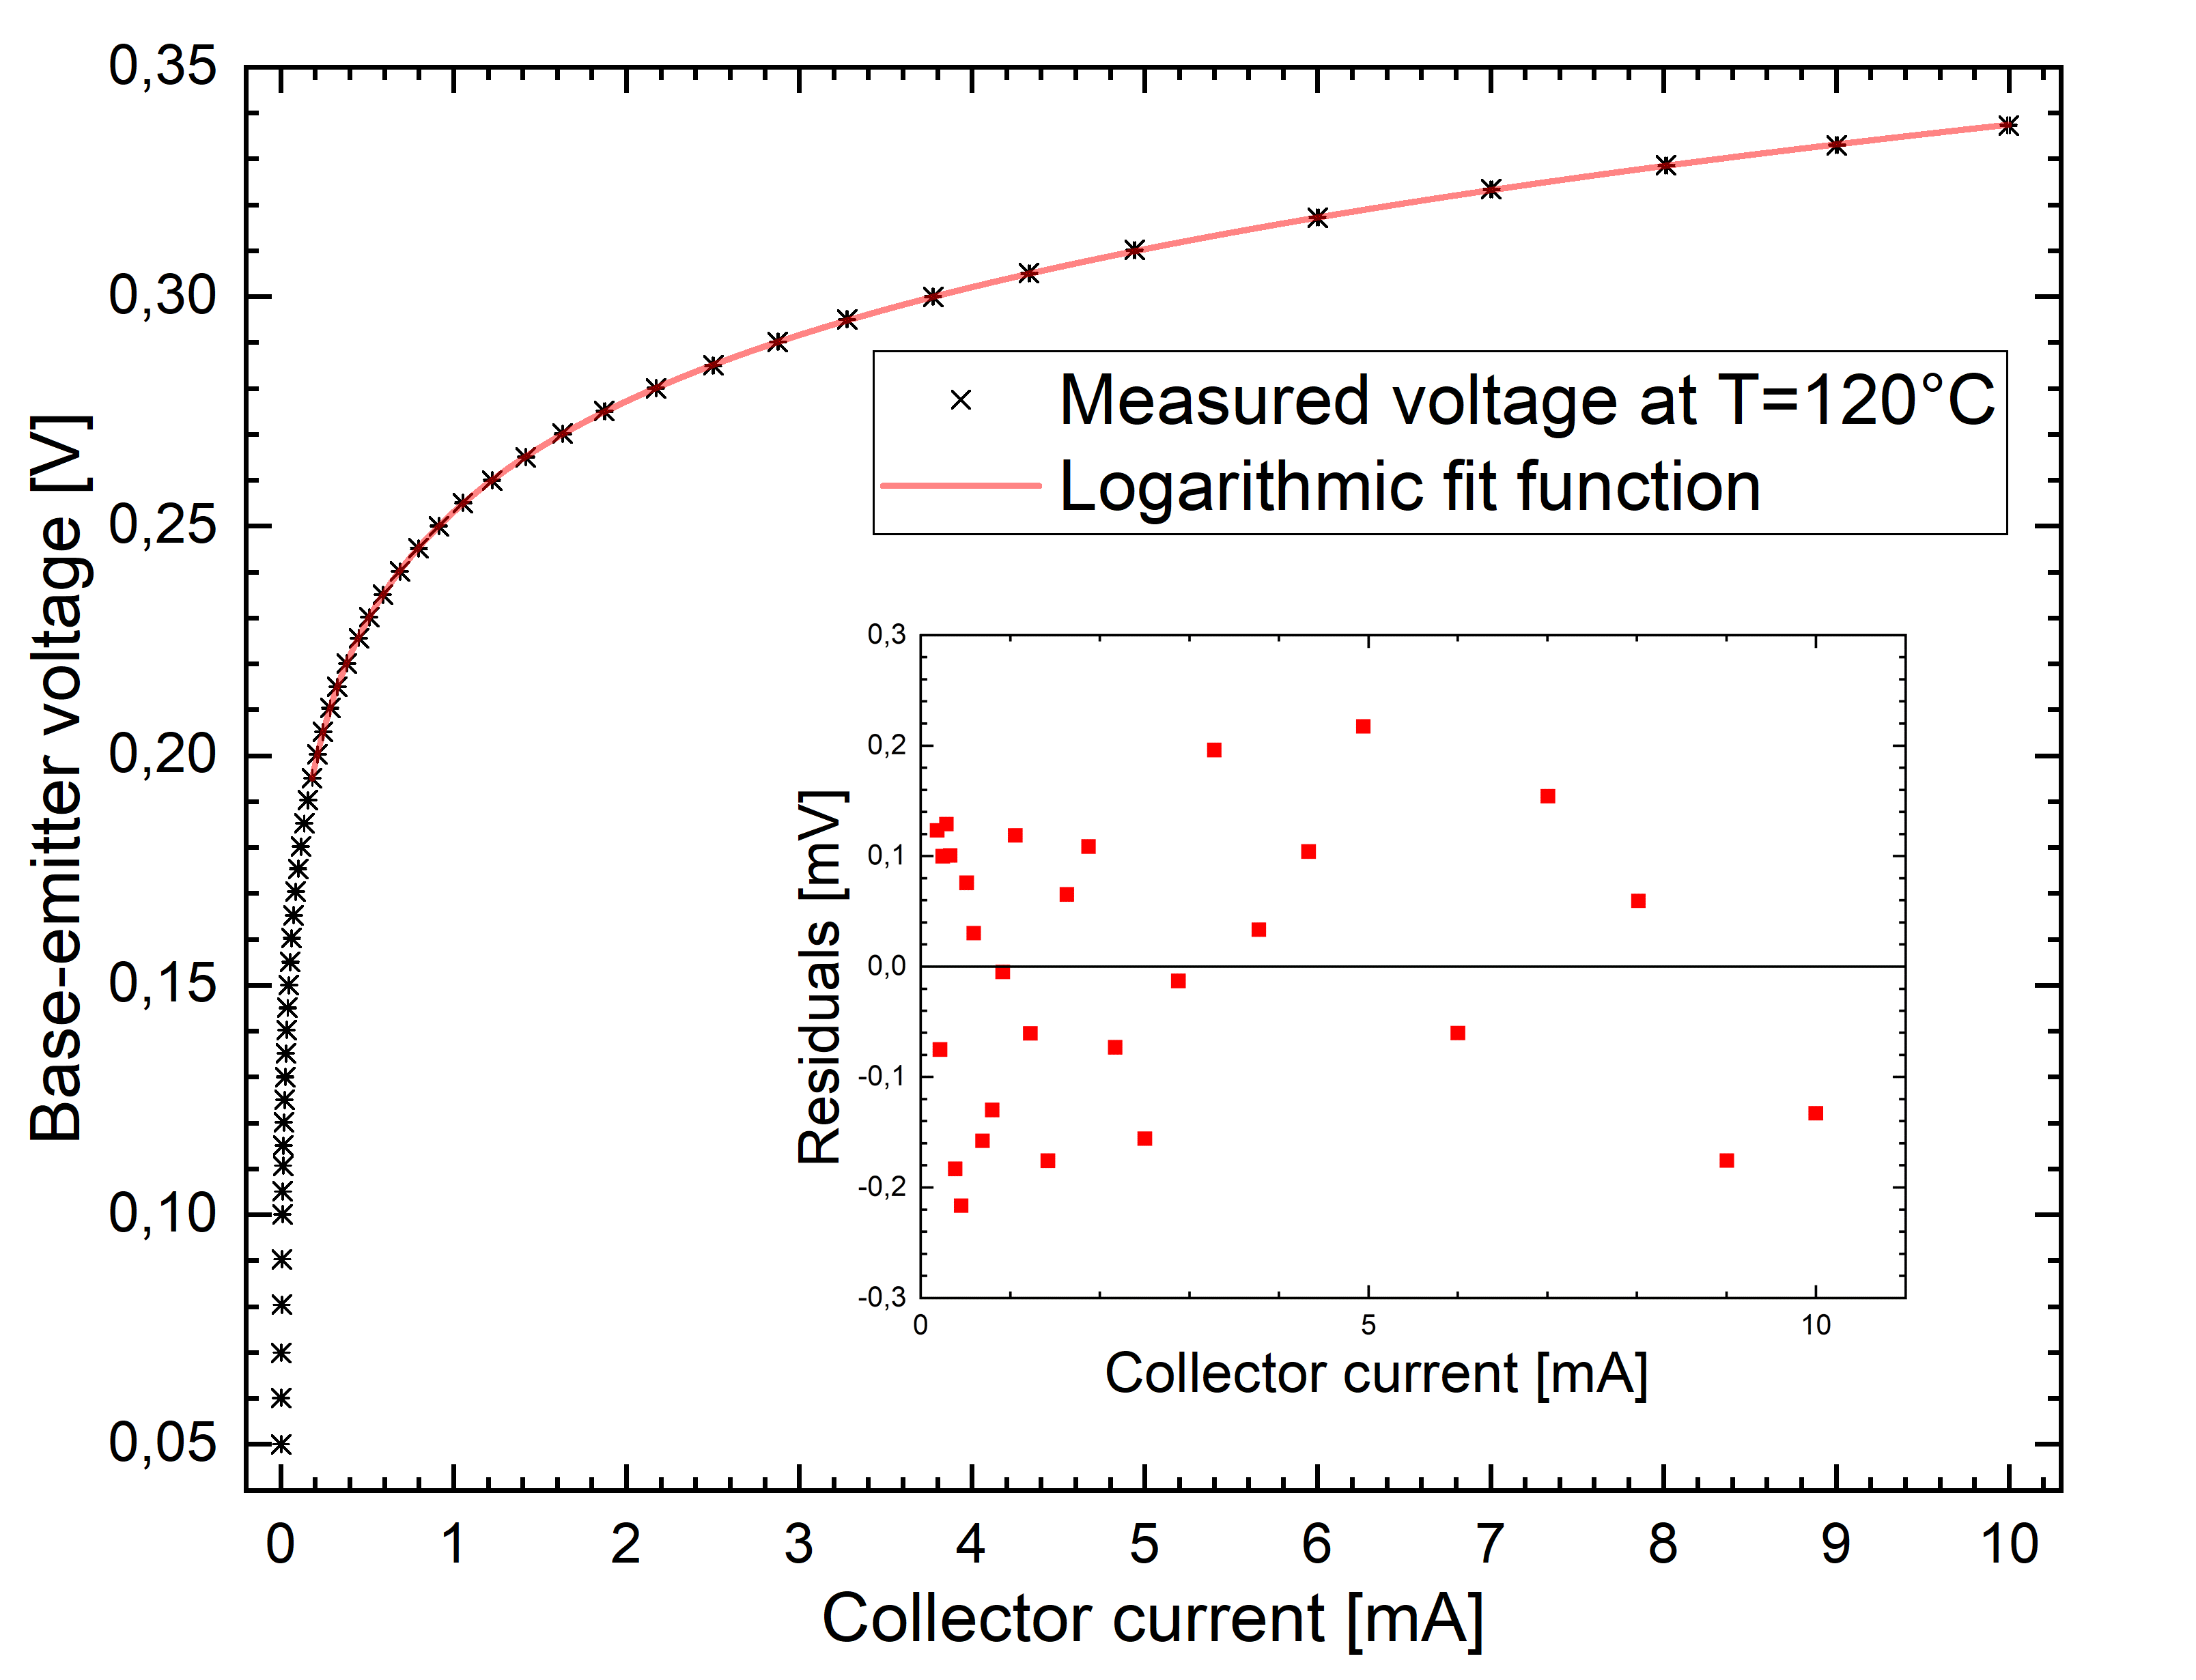
\includegraphics[width=\columnwidth]{img/R_120C}
\end{center}
\caption[]{Determination of the emitter-resistance by plotting the base-emitter voltage against the collector current, so the parameters of a logarithmic fit function give us the resistance.}
\label{fig:boltzmann-120R}
\end{figure}
Now, we can fit a logarithm to this data and determine the value for $R$, as is shown in Fig.~\ref{fig:boltzmann-120R}. With this value, we can now correct our voltage values $U$ and these corrected voltages with the corresponding currents are then finaly fitted with an exponential function following eq.~\ref{eq:schockley0}, such that the Boltzmann constant as well as its error can be calculated from the fit parameters (see Fig.~\ref{fig:boltzmann-120-1} and~\ref{fig:boltzmann-40-80-1}). As in the correction step we can not take the current errors into account, we only use datapoints where the relative error of the current is less than $1\%$. The three values as well as the final weighted mean are given in Tab.~\ref{tab:boltzmann}.
\begin{figure}[htbp]
\begin{center}
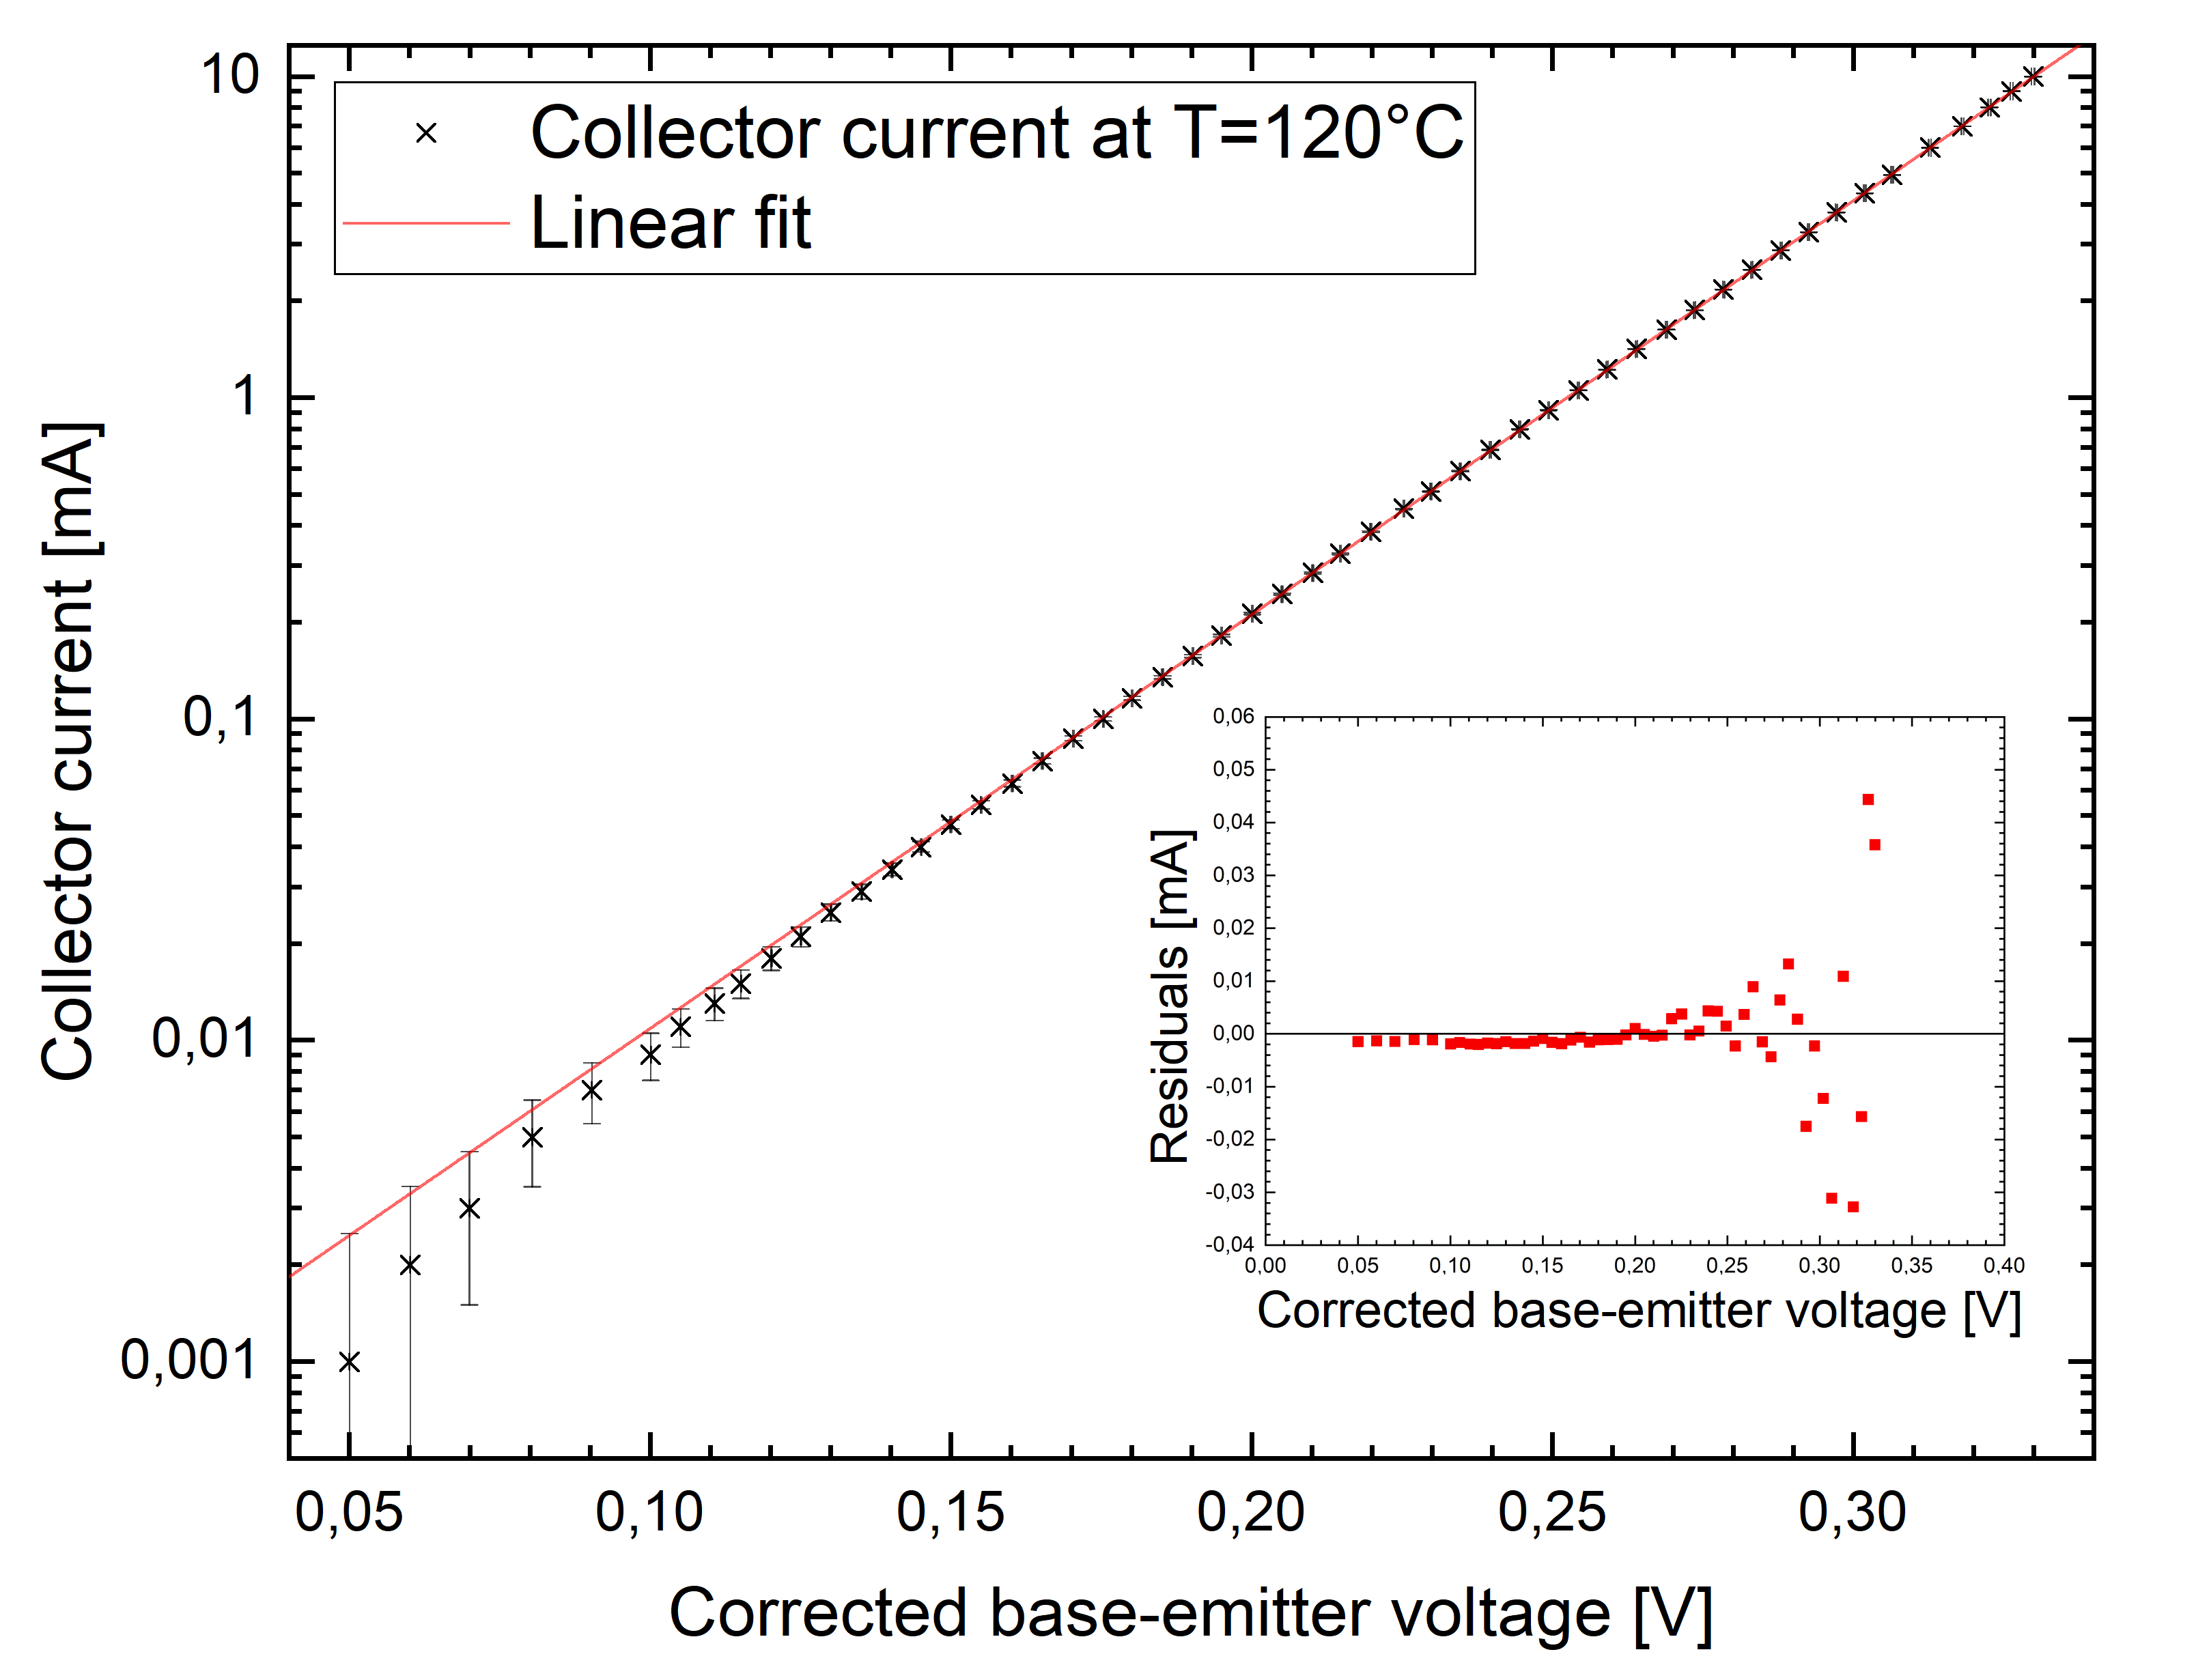
\includegraphics[width=\columnwidth]{img/120C_Kennlinie_korr_1}
\end{center}
\caption[]{Collector current in dependence of the corrected base-emitter voltage at temperature $T=120\,\si\celsius$ in logarithmic application with a linear fit function.
As the emitter-resistance is accounted for, the data follows the linear expectation quite well. From the slope of this line, the Boltzmann constant can be calculated.}
\label{fig:boltzmann-120-1}
\end{figure}
\begin{table}[htbp]          %so funktionieren die Tabellen in LaTeX
\centering
\begin{tabular*}{\linewidth}{@{\extracolsep{\fill}}cc}
\hline
\hline
\rule[-7pt]{0pt}{23pt} \small Temperature $T$ [$\si{\celsius}$]  & \small Boltzmann constant $k_\text B$ [$10^{-23}\frac{\si\J}{\si\K}$]  	 \\
\hline
\rule[-5pt]{0pt}{23pt}   $40,0 \pm 0,4$   &   $1,3854 \pm 0,0024$ 	 \\
\rule[-5pt]{0pt}{23pt}   $80 \pm 0,4$   &   $1,3778 \pm 0,0021$  	 \\
\rule[-5pt]{0pt}{23pt}   $120 \pm 0,4$   &   $1,3736 \pm 0,0017$  	 \\
\hline
\rule[-5pt]{0pt}{23pt}   mean value   &   $1,3777 \pm 0,0012$  	 \\
\hline
\hline
\end{tabular*}  
\normalsize
\caption[]{Values for the Boltzmann constant obtained at different temperatures and the mean value.}  %siehe Graphik: Beschriftung
\label{tab:boltzmann}                             %siehe Graphik: zum Zitieren
\end{table}
\\\\Our value of $k_\text B=(1,3777 \pm 0,0012)\cdot 10^{-23}\,\frac{\si J}{\si K}$ deviates from the exact value of $k_\text{B, exact}=1,380649\cdot 10^{-23}\,\frac{\si J}{\si K}$ \cite{codata} by $0,2\%$. As this deviation is quite small, the fact that the values do not coincide within the margin of error is most likely because our error was estimated too small. This happened during the correction of the base-emitter voltage, where we were not able to include the current errors into the nonlinear fit.


\section{Conclusion}
In this paper, we measured the values for Planck's and Boltzmann's constants. We used the photoelectric effect and measured the energy of the photoelectrons at different light frequencies, from which we then received Planck's constant as $h=(5,75\pm0,51)\,\cdot10^{-34}\,\si Js$. This value does not coincide with the exact value within the margin of error, but is well within the two-sigma interval.\\ Boltzmann's constant was obtained by measuring the diffusion current at a pn-transition inside of a transistor. As in thermal equilibrium this current follows a Boltzmann factor, we could interpolate our data and calculate the constant from the fit parameters to be $k_\text B=(1,3777 \pm 0,0012)\cdot 10^{-23}\,\frac{\si\J}{\si\K}$. This value does not coincide with the exact value for Boltzmann's constant within the margin of error, which can be explained by some errors we had to neglect during the data analysis, but the values differ by less than half a percent, which is well within our expectation for a realistic error.

\FloatBarrier

%FF: Angabe der verwendeten Literatur mit Quellennachweis.
\begin{thebibliography}{}    %so wird das Literaturverzeichnis erstellt
\bibitem{instr} Physikalisches Grundpraktikum, Universit�t W�rzburg, Modul C2, Versuch 45, \grqq Plancksches Wirkungsquantum 
und Boltzmann-Konstante\grqq, 2021 
\bibitem{gerth} Meschede, Dieter, Gerthsen Physik, 25. Auflage, Springer-Verlag, Berlin, 2015 
\bibitem{codata} E. Tiesinga \textit{et al.}, \grqq CODATA
recommended values of the fundamental physical constants: 2018\grqq, Rev. Mod. Phys. 93, 025010 (2021)

\end{thebibliography}


\newpage\,\newpage
\section{Appendix}

\subsection{Interpolation of the electron energies in the planck data}\label{sec:planck-int}
In the $I(U)$ curve we can see the linear ascending background signal as well as the photocurrent added on top of it. As we are interested in the voltage where the photocurrent becomes nonzero, we want to find the kink in the data where the points are no longer linearly ascending. To do so, we define a function
\begin{align}
f(x):=\left\{%
\begin{array}{ll}
    A+M(x-U) & \hbox{for x $\leq$ U} \\
    A+B(e^{C(x-U)}-1) & \hbox{else} \\
\end{array}%
\right.
\end{align}
and fit it to the data. The linear part models the underground while the exponential is just an unphysical fit that approximately describes the observed data. The parameter U gives us the transition point from underground to photocurrent, thus the maximum voltage a photoelectron can overcome, which is used in further evaluation. These fits can be found in fig.~\ref{fig:planck-prim1} and \ref{fig:planck-prim2-5}.
\begin{strip}
\subsection{Plots analysing the Planck data}
\begin{center}
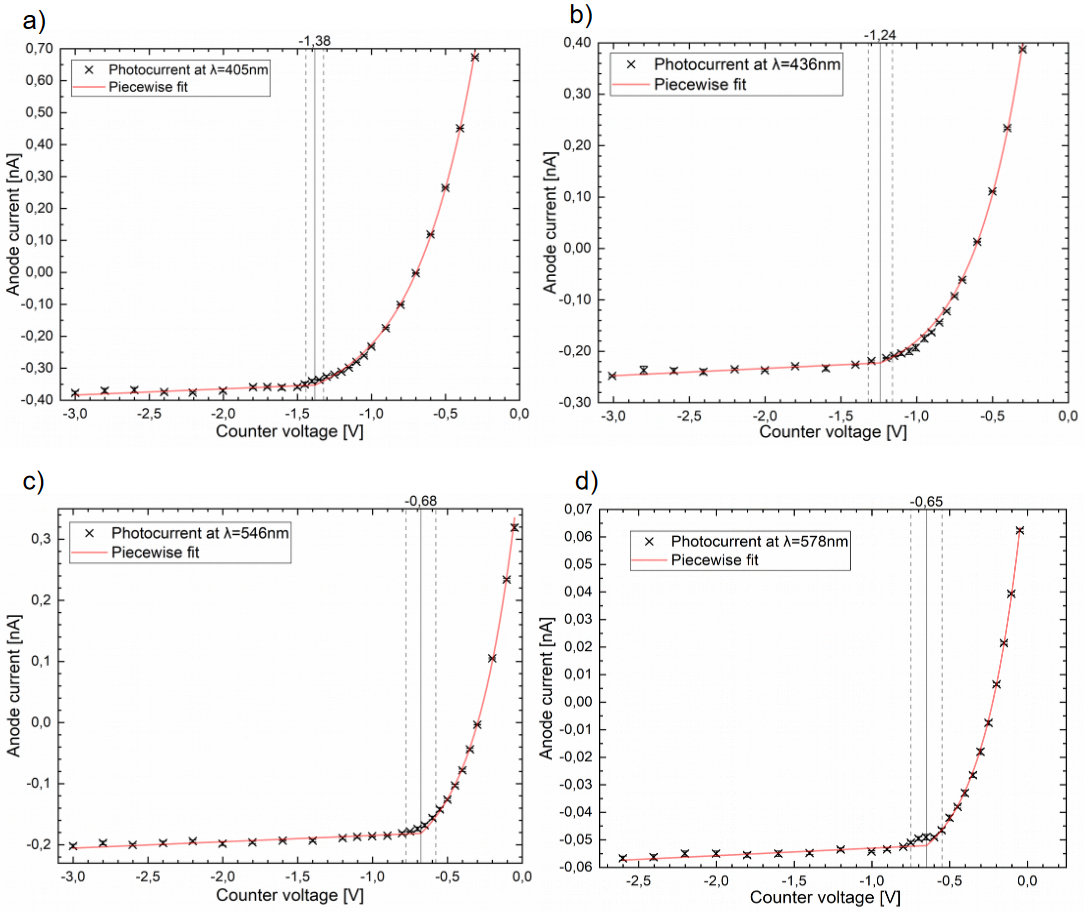
\includegraphics[width=2\columnwidth]{img/Planck-prim-2-5}
\end{center}
\vspace{-10ex}
\captionof{figure}{\label{fig:planck-prim2-5}Photocurrent in dependence of the countervoltage for light of wavelengths a) $\lambda= 405 \,\si\nm$, b) $\lambda= 436 \,\si\nm$, c) $\lambda= 546 \,\si\nm$ and d) $\lambda= 578 \,\si\nm$. Piecewise functions (first linear and then exponential) were fitted to the data to determine the points where the relevant signal is detectable against the underground. These are at the transition points between the two functions.}


\subsection{Plots analysing the Boltzmann data}
\begin{center}
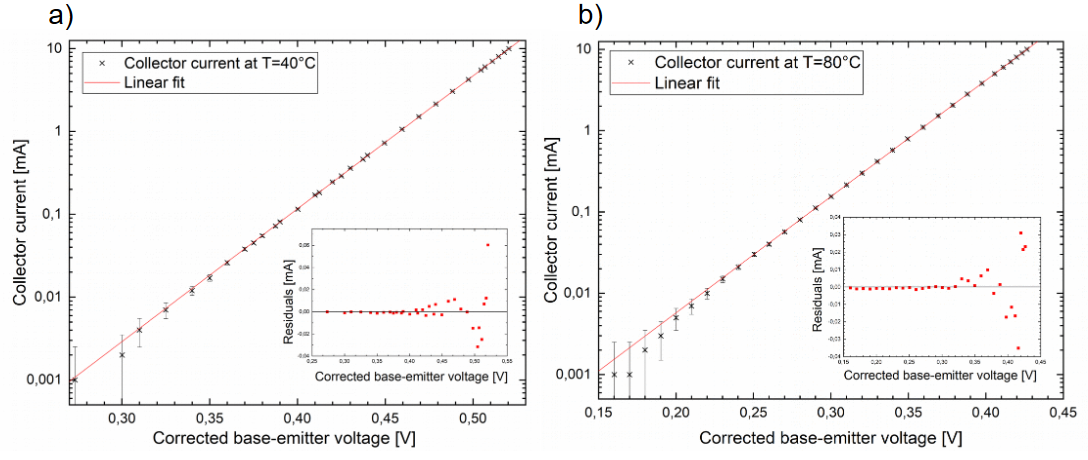
\includegraphics[width=2\columnwidth]{img/Boltzmann-40-80_korr1}
\end{center}
\captionof{figure}{\label{fig:boltzmann-40-80-1}Collector current in dependence of the corrected base-emitter voltage at temperature a) $T=40\,\si\celsius$ and b) $T=80\,\si\celsius$ in logarithmic application with a linear fit function.
As the emitter-resistance is accounted for, the data follows the linear expectation quite well. From the slope of these lines, the Boltzmann constant can be calculated.}
\end{strip}

\end{document}




